\section{Towards General Data Management Policies}
\label{sec:scope}

%\begin{itemize}
%  \item Lustre Trace
%  \item LinkedIn Trace
%  \item Nathan's Trace
%\end{itemize}

In the previous section, we used our data management language and the Mantle
policy engine to design effective cache management strategies for a new service
and domain. In this section, we compare and contrast the policies examined for
file system metadata load balancing in~\cite{sevilla:sc15-mantle} with the ones
designed for cache management in ParSplice. The similarities show how the
``when"/``where"/``how much" abstractions, data management language, and policy
engine may be widely applicable to other data management techniques, such as
QoS, scheduling, and batching.

\subsection{Using File System Policies for ParSplice}

%- memory utilization/heuristics
From a high-level the cache management policy we designed in
Figure~\ref{src:lru-dyn} trims the cache if the cache reaches a certain size
{\it and} if it has already absorbed the initial burstiness of the workload.
Much of this implementation was inspired by the file system metadata load
balancing policy in Figure~\ref{src:lua-cephfs}, which was presented
in~\cite{sevilla:sc15-mantle}. That policy migrates file system metadata if the
load is higher than the average load in the cluster {\it and} the current
server has been overloaded for more than two iterations. The two policies have
the following in common:

\textbf{Condition for ``Overloaded"} (Fig.~\ref{src:lru-dyn}: Line 2;
Fig.~\ref{src:lua-cephfs}: Line 2) - these lines detect whether the node is
overloaded using the load calculated in the load callback (not shown). While
the calculations and thresholds are different, the way the loads are used is
exactly the same; the ParSplice policy flags the node as overloaded if the
cache reaches a certain size while the CephFS policy compares the load to other
nodes in the system.

\textbf{State Persisted Across Decisions} (Fig.~\ref{src:lru-dyn}: Lines 4,6;
Fig~\ref{src:lua-cephfs}: Lines 3,4,10) - these lines use Mantle to write/read state
from previous decisions.  For ParSplice, we save a boolean that indicates
whether we have absorbed the workload's initial burstiness. For CephFS, we save
the number of consecutive instances that the server has been overloaded. We
also clear the count (Line 10) if the server is no longer overloaded. 

\textbf{Two-Part Policies} (Fig.~\ref{src:lru-dyn}: Line 6;
Fig.~\ref{src:lua-cephfs}: Line 5) - after determining that the node is
overloaded, these lines add an additional condition before the policy enters a
data management state.  ParSplice trims its cache once it eclipses the
``absorb" threshold while CephFS allows balancing when overloaded for more than
two iterations. The persistent state is essential for both of these
policy-switching conditions.

\begin{figure}[t]
\footnotesize
\begin{minted}[xleftmargin=3em,linenos]{lua}
local function when()
  if servers[whoami]["load"] > target then
    overloaded = RDstate() + 1
    WRstate(overloaded)
    if overloaded > 2 then
      return true
    end
  end
  else then
    WRstate(0)
  end
  return false
end
\end{minted}
\caption{CephFS file system metadata load balancer.\label{src:lua-cephfs}}
\end{figure}

\subsection{Using ParSplice Policies for File Systems}

%- how many inodes to keep in mds/client caches
%- affects LB; increases capacity of single MDS (reduces req/mem pressure)
%- affects LB; tells us which part of the cache to keep local

% Load balancing in FSs
Mantle was designed for file system metadata load balancing across a cluster of
dedicated metadata servers, where spreading requests across servers improves
performance. But another technique to reduce request load is caching. If
clients and servers maintain a consistent cache, the client can do operations
locally without contacting the metadata server.  The caches in CephFS have the
same performance and utilization trade-off as ParSplice, where large caches
improve performance at the expense of a higher memory footprint. High memory
utilization is problematic when a single metadata server maintains consistent
caches with many clients.  Using cache management policies from the previous
two sections has two benefits for load balancing: (1) increases the capacity of
a single metadata server, and (2) helps identify which parts of the cache to
keep local to a server. For example, applying the keyspace access pattern
detection algorithm from Section~\S\ref{sec:regime-detection} to a similar file
system access pattern has the potential to identify when to migrate keys and
how many keys to migrate.

% burstiness of creates then compile
To explore this example in more detail, consider the trace of metadata requests
for compiling code in CephFS shown in Figure~\ref{fig:compile-ops}.  That trace
shows the number of file system metadata requests serviced by the metadata
server when uncompressing (\texttt{untar}), compiling (\texttt{make}), and
deleting (\texttt{rm}) the source code for the Linux kernel. If the system
knows that the job phases would progress from many creates, to many lookups, to
many deletes, then it could size its caches accordingly. For example, the file
system could cache none of the metadata from the \texttt{untar} phase and run
regime detection during the \texttt{make} phase, resulting in the metadata
server/clients only caching metadata that is repeatedly used. For the job in
Figure~\ref{fig:compile-ops}, this would fill up the cache to only 20K inodes
(the unit of metadata for file systems) instead of 60K, resulting in almost
40MB of memory savings (since an inode is about
1KB\footnote{http://docs.ceph.com/docs/master/dev/mds\_internals/data-structures/})
without sacrificing performance.

%- strategy: cache all inodes on create
\begin{figure}[t]
\noindent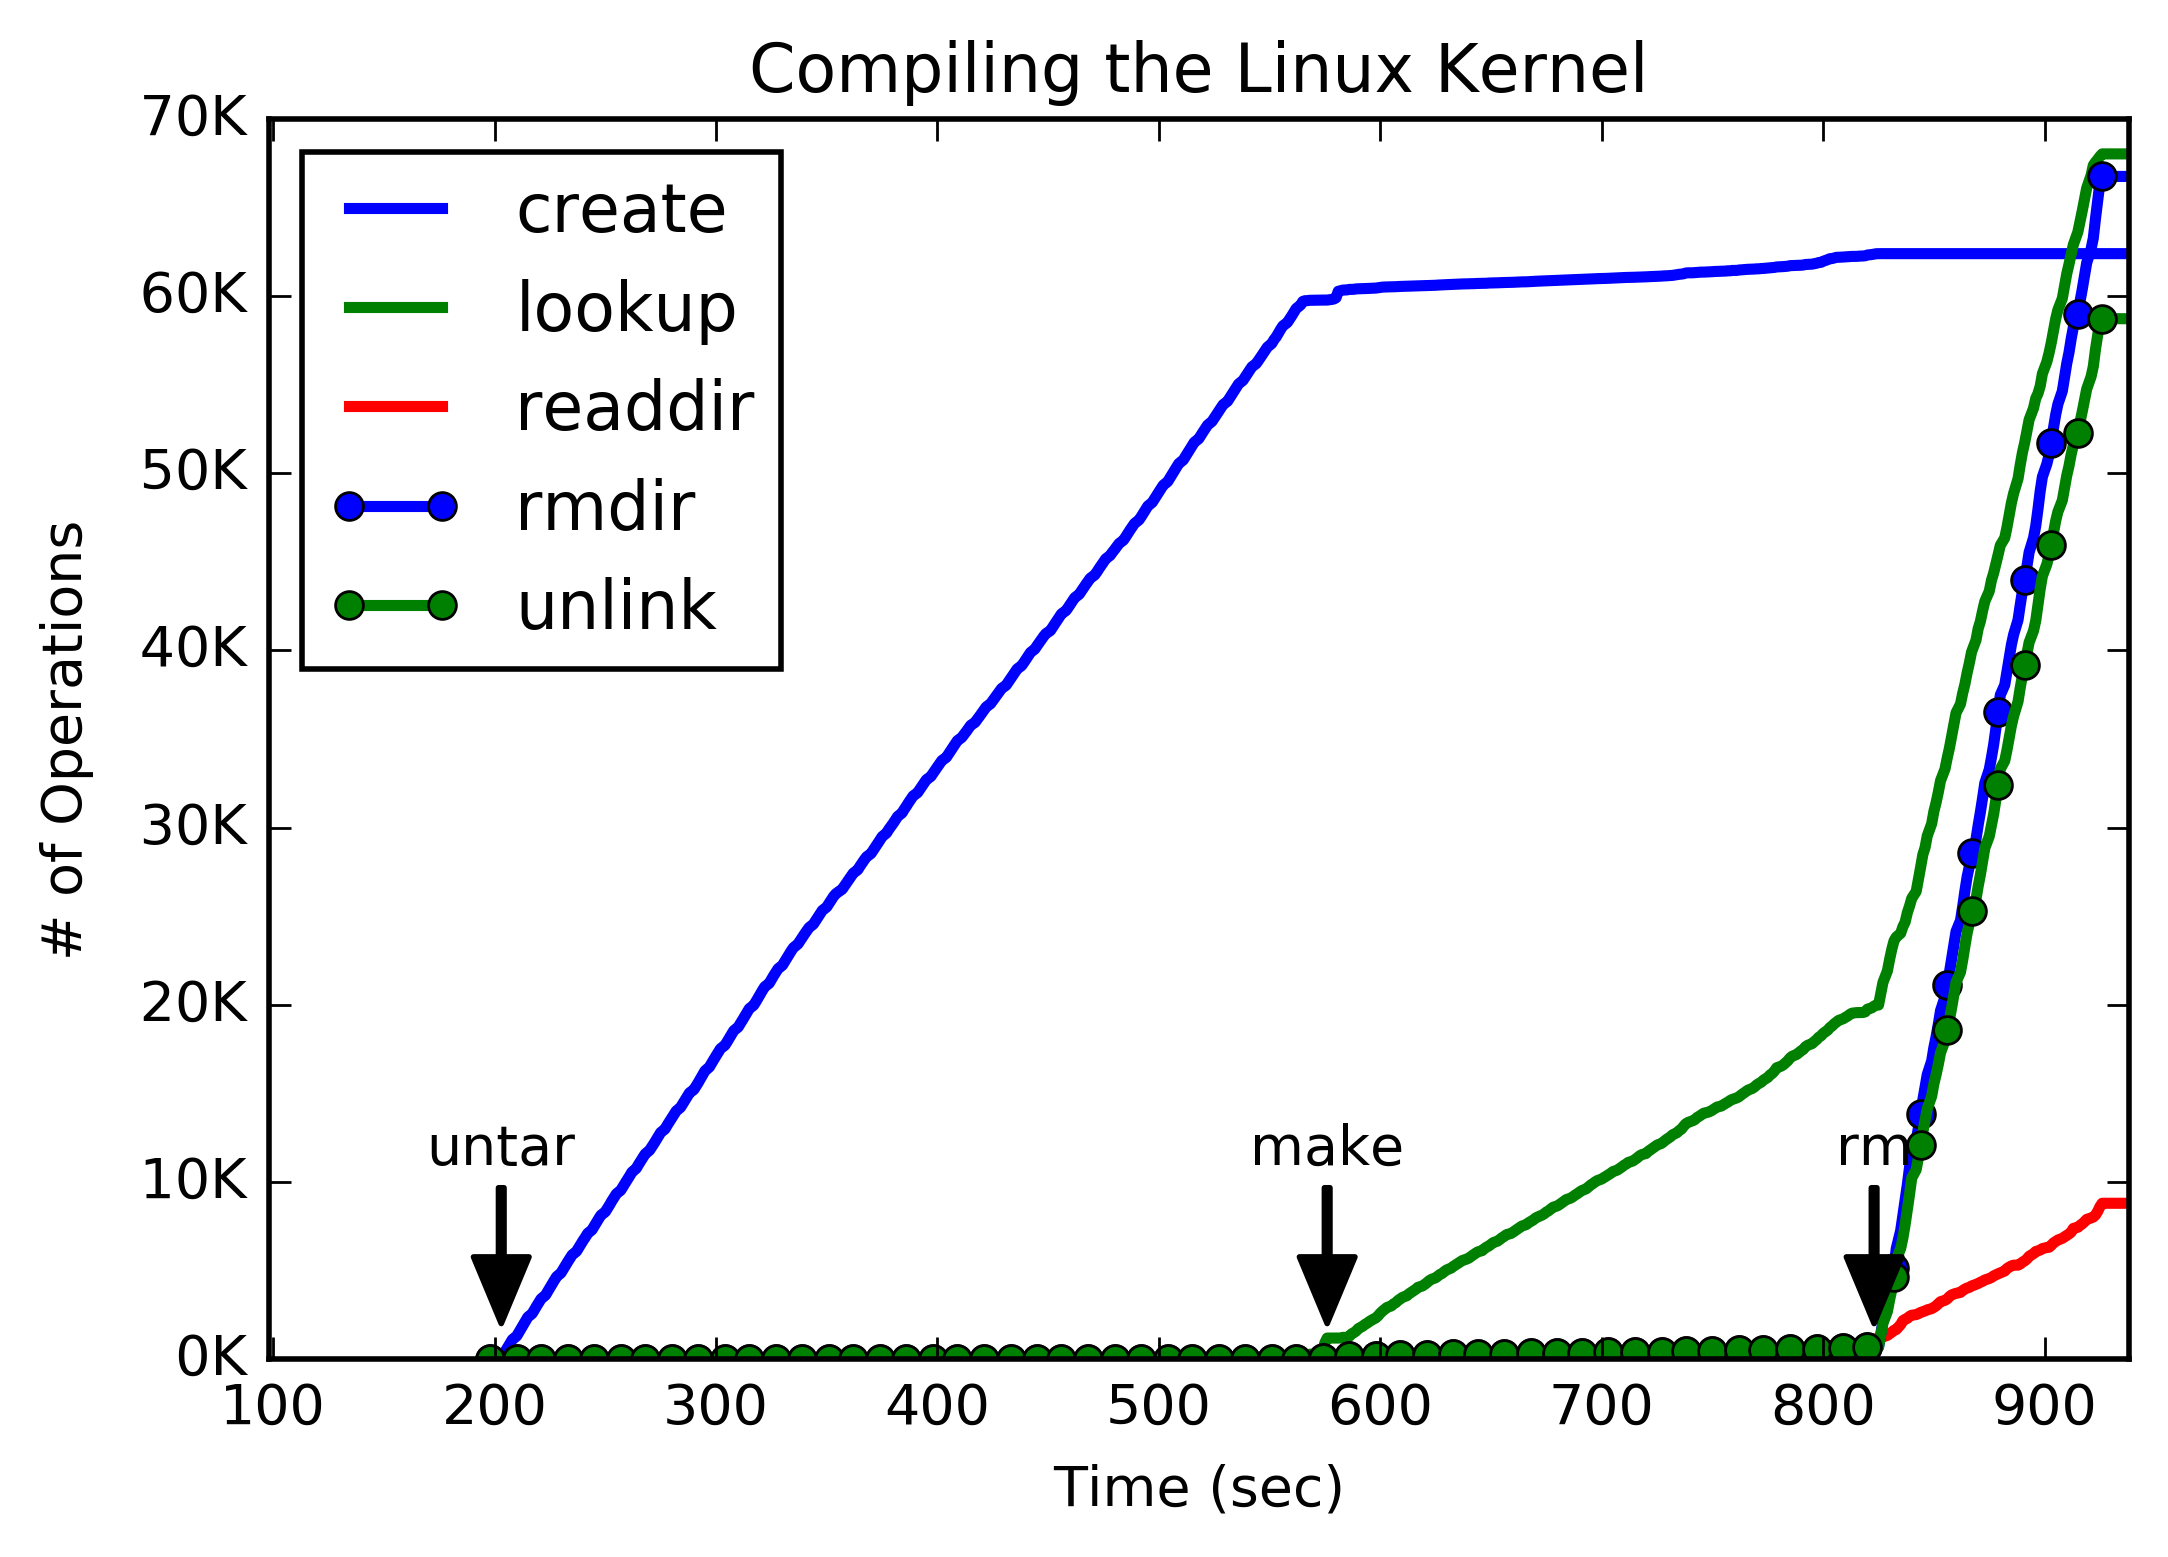
\includegraphics[width=0.5\textwidth]{figures/compile-ops.png}\\
\caption{The file system metadata requests for a compile job shows distinct
workload phases, characterized by a dominant request type ({\it e.g.}, creates
for ``untar", lookups for ``make", etc.). Using a ParSplice cache management
policy for a workload like this in file systems could reduce memory pressure
without sacrificing performance.  \label{fig:compile-ops}}
\end{figure}

% other use cases caches/tiers 
Ceph has many other data management techniques that would benefit from the
caching policies developed in Sections~\S\ref{sec:arch-specific}
and~\ref{sec:dom-specific}. Administrators can use the policies in ParSplice to
automatically size and manage cache
tiers\footnote{http://docs.ceph.com/docs/master/rados/operations/cache-tiering/},
caching on object storage devices, or in the distributed block
devices\footnote{http://docs.ceph.com/docs/master/rbd/rbd-config-ref/}.
Integration with Mantle would be straightforward as it is merged into Ceph's
mainline\footnote{http://docs.ceph.com/docs/master/cephfs/mantle/} and the
three caching subsystems mentioned above already maintain keyspace access
traces. We hypothesize that since this is all software defined caching,
something more clever than LRU would improve cache utilization without
sacrificing too much performance.

\subsection{Other Use Cases}
% we said this is good for LB/Cache management... what about others??
% QoS: when to move clients, where to move clients, how much of the reservation to move
% Other cache management: MRU
% Scheduling: how much of a resource to allocate; more than just LRU (RAD)
%\subsection{Visualizing File System Traces like ParSplice Keyspace Traces}

